% --------------------------------------------------------------------------------

\begin{exercise}

Seien $\Omega \subset \R^n$ ein beschränktes Gebiet und $f:\R \times \overline{\Omega} \to \R$ stetig und im ersten Argument stetig differenzierbar mit $f_u(u, x) \geq 0$ für alle $(u, x) \in \R \times \Omega$, und $\varphi \in C(\overline{\Omega})$.

\begin{enumerate}[label = (\alph*)]

  \item Zeigen Sie, dass

  \begin{align*}
    \Delta u = f(u, x) ~\text{in}~ \Omega,
    \quad
    u = \varphi ~\text{auf}~ \partial \Omega
  \end{align*}

  höchstens eine klassische Lösung besitzt
  (\textit{Hinweis:} Mittelwertsatz der Differentialrechnung).

  \item Finden Sie für $n = 1$ ein Intervall $\Omega \subset \R$ und eine Funktion $f \in C^1(\R)$ mit $f^{\prime}(u) < 0$ für alle $u$ so, dass

  \begin{align*}
    u^\primeprime = f(u) ~\text{in}~ \Omega,
    \quad
    u = 0 ~\text{auf}~ \partial \Omega
  \end{align*}

  nicht eindeutig lösbar ist.

\end{enumerate}

\end{exercise}

% --------------------------------------------------------------------------------

\begin{solution}

\phantom{}

\begin{enumerate}[label = (\alph*)]

  \item Seien $u_1$ und $u_2$ klassische Lösungen und $u := u_1 - u_2$.
  Laut dem Mittelwertsatz der Differentialrechnung $\Exists \vartheta: \R \times \R \to (0, 1):$

  \begin{multline*}
    \Delta u(x)
    =
    \Delta u_1(x) - \Delta u_2(x)
    =
    f(u_1(x), x) - f(u_2(x), x) \\
    =
    \underbrace
    {
      f_u(\vartheta(u_1(x), u_2(x)) - (1 - \vartheta (u_1(x), u_2(x)) u_2(x)), x)
    }_{
      =: c(x)
    }
    \underbrace
    {
      (u_1(x) - u_2(x))
    }_{
      u(x)
    }
  \end{multline*}

  Wir betrachten nun den Differentialoperator $L := -\Delta + c$.
  $u$ erfüllt also das folgende RWP.

  \begin{align*}
    Lu = 0 ~\text{auf}~ \Omega,
    \quad
    u = 0 ~\text{auf}~ \partial \Omega
  \end{align*}

  Laut Voraussetzung ist $c \geq 0$.

  \begin{align*}
    \Forall (u, x) \in \R \times \Omega:
    f_u(u, x) \geq 0
    \implies
    c \geq 0
  \end{align*}

  Wir können also Satz 5.27 (Schwaches Maximumprinzip für $c \geq 0$) auf das konstruierte RWP anwenden.

  \includegraphicsboxed{PDEs/PDEs_-_(5-20).png}

  \begin{center}
    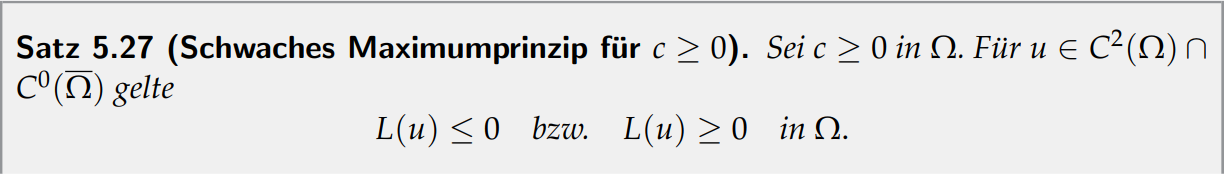
\includegraphics[width = 0.75 \textwidth]{PDEs/PDEs_-_Satz_5-27-1_(Schwaches_Maximumprinzip_fuer_c_geq_0).png}
    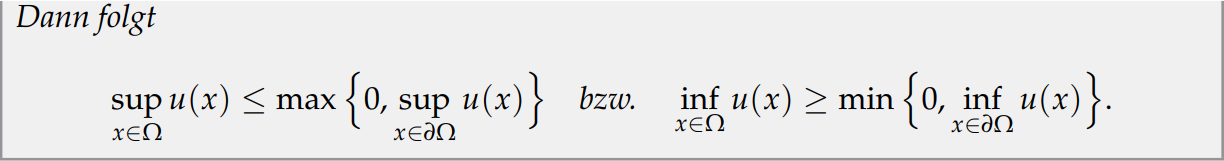
\includegraphics[width = 0.75 \textwidth]{PDEs/PDEs_-_Satz_5-27-2_(Schwaches_Maximumprinzip_fuer_c_geq_0).png}
  \end{center}

  \begin{align*}
    & \implies
    \inf_{x \in \partial \Omega} u(x)
    =
    \sup_{x \in \partial \Omega} u(x)
    =
    0 \\
    & \implies
    0
    =
    \min \Bbraces{0, \inf_{x \in \partial \Omega} u(x)}
    \leq
    \inf_{x \in \Omega} u(x)
    \leq
    \sup_{x \in \Omega} u(x)
    \leq
    \max \Bbraces{0, \sup_{x \in \partial \Omega} u(x)}
    =
    0 \\
    & \implies
    u = 0 \\
    & \implies
    u_1 = u_2
  \end{align*}
  \item
  \begin{align*}
    \Omega = (0, \pi),
    \quad
    f := -\id,
    \quad
    u_\pm := \pm \sin
  \end{align*}

\end{enumerate}

\end{solution}

% --------------------------------------------------------------------------------
